\chapter{Critical behavior within 20 fs drives the out-of-equilibrium laser-induced magnetic phase transition in nickel}
\label{Critical Behavior}

In this chapter we describe experiments carried out on single crystal nickel (111). Although this material was in fact the first one where ultrafast laser-induced demagnetization was observed, many things about that process are still poorly understood. In this study, we compare the results of time resolved transverse magneto optical Kerr effect spectroscopy and angle resolved photoemission spectroscopy both using extreme ultraviolet light from high harmonic generation. By comparing the results of these two experimental techniques, we are able to gain fundamental new insights about the laser-induced demagnetization process and show that the same critical behavior that dominates the static temperature-driven magnetic phase transition also governs the ultrafast phase transition in nickel.

It has long been known that ferromagnets undergo a phase transition from ferromagnetic to paramagnetic at the Curie temperature, associated with critical phenomena such as a divergence in the heat capacity. A ferromagnet can also be transiently demagnetized by heating it with an ultrafast laser pulse. However, to date, the connection between out-of-equilibrium and equilibrium phase transitions, or how fast the out-of-equilibrium phase transitions can proceed, was not known. By combining time- and angle-resolved photoemission with time-resolved transverse magneto-optical Kerr spectroscopies, we show that the same critical behavior also governs the ultrafast magnetic phase transition in nickel. This is evidenced by several observations. First, we observe a divergence of the transient heat capacity of the electron spin system preceding material demagnetization. Second, when the electron temperature is transiently driven above the Curie temperature, we observe an extremely rapid change in the material response: The spin system absorbs sufficient energy within the first 20 fs to subsequently proceed through the phase transition, whereas demagnetization and the collapse of the exchange splitting occur on much longer, fluence- independent time scales of ~176 fs. Third, we find that the transient electron temperature alone dictates the magnetic response. Our results are important because they connect the out-of-equilibrium material behavior to the strongly coupled equilibrium behavior and uncover a new timescale in the process of ultrafast demagnetization.

\section{Introduction}

In this chapter, we present clear evidence that critical behavior on a new ultrafast 20 fs time scale governs laser induced demagnetization in nickel. We show this by correlating time- and angle-resolved photoelectron spectroscopy (Tr-ARPES) with Tr-TMOKE spectroscopy, as well as with EUV transient reflectivity, all using tabletop high-harmonic sources \cite{La-O-Vorakiat2012}. Through fluence and temperature dependent studies, we make several surprising observations. First, we observe critical behavior as the spin system undergoes a transient magnetic phase transition: As the laser fluence approaches a critical fluence $F_c$ of $\approx$2.8 mJ/cm$^2$,cor- responding to a hot electron temperature approaching the Curie temperature (631 K), significantly more laser energy is required to increase the peak electron temperature, indicating a divergence in the heat capacity of the spin system. Second and very surprisingly, the spin system absorbs sufficient energy within the first 20 fs to subsequently proceed through the phase transition. This defines a new time scale in the process of ultrafast demagnetization. Demagnetization (measured using TMOKE) and the collapse of the exchange splitting (measured using ARPES) both occur on much longer and similar timescales of 176 fs, independent of the laser fluence. Third, the recovery dynamics of the exchange splitting also exhibit a critical behavior, changing from a full recovery within 500 fs when pumped at fluences below $F_c$ to a much longer 76-ps recovery above $F_c$. These critical phenomena indicate that the transient electron temperature alone dictates the magnetic response.

We note that our findings are in contrast to past work assuming that the electron bath alone absorbs the laser energy, which is then slowly transferred to the spin system throughout the demagnetization process \cite{Koopmans2010,Bigot2009,Mueller2013,Roth2012}. Instead, our results imply that the ultrafast demagnetization of a ferromagnetic metal is driven by a highly nonequilibrium process that takes place within the first 20 fs, with sufficient energy transfer from the optical excitation to the spin system to subsequently proceed through the transient magnetic phase transition (see Fig. 1). This ultrafast, highly nonequilibrium process can likely be driven by superdiffusive spin currents (10, 11) or spin mixing via spin-orbit coupling \cite{Tows2015,Zhang2012,Krieger2015}. Then, demagnetization of the sample occurs on a longer time scale of 176 fs, likely mediated by processes such as low-energy magnon generation.

\section{Results}

The observed critical behavior in laser-induced ultrafast demagnetization in nickel is shown schematically in Fig. \ref{fig: Nifig1}A. Our time-resolved ARPES and TMOKE measurements were both performed using 780-nm laser-driven EUV high-harmonic generation (HHG) probe beams, as shown in Fig. \ref{fig: Nifig1} (B and C) (see Materials and Methods). For all measurements, the sample used is a 400-nm Ni(111) single-crystalline film grown on an $\alpha-Al_{2}O_{3}$(0001) substrate \cite{Miller2012}. The Ni film thickness is much greater than both the pumping (13 nm) and probing depth (1 nm for ARPES; 10 nm for TMOKE) to avoid any influence of the substrate, capping layer, or multilayer structure \cite{Rudolf2012, Dakovski2016,Eschenlohr2013}. 

\begin{figure}[htbp]
	\label{fig: Nifig1}
	\begin{center}
		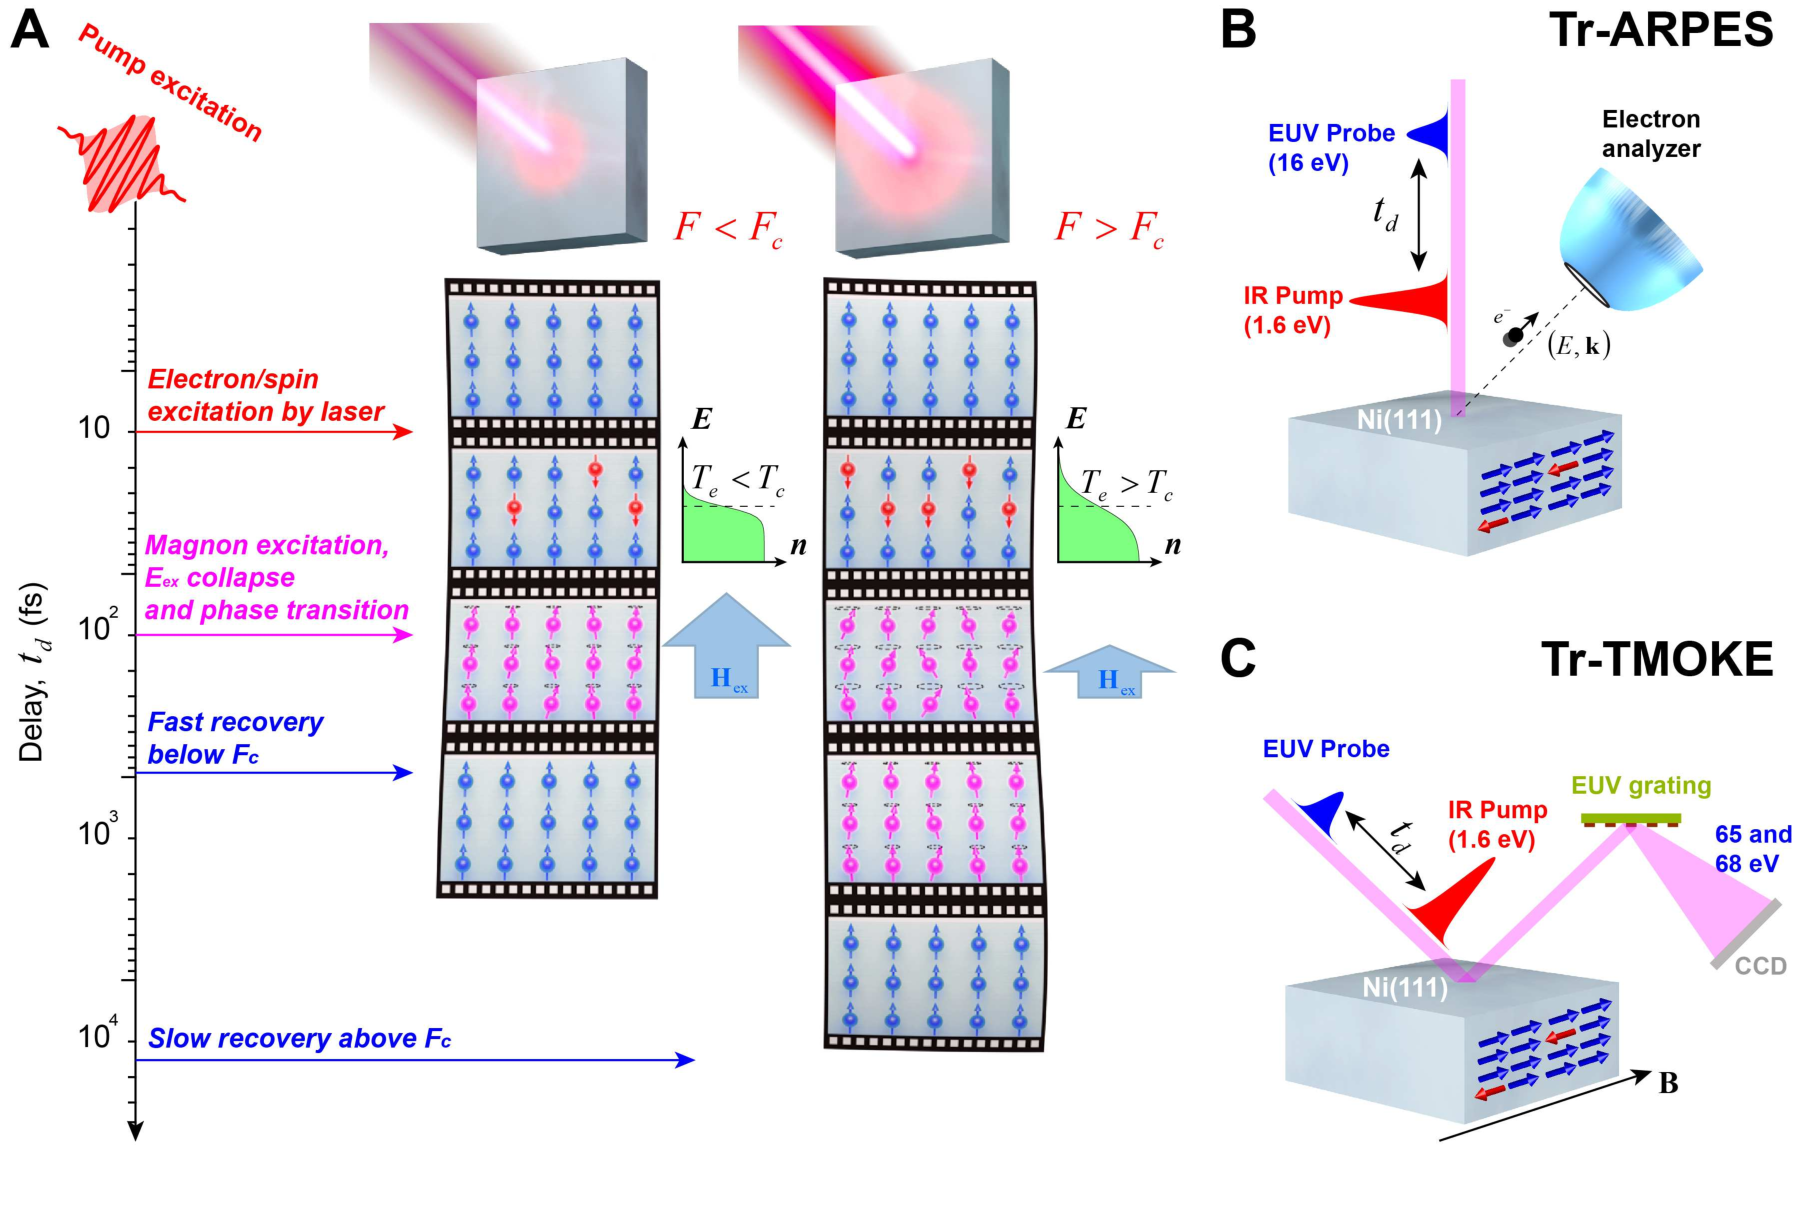
\includegraphics[width=150mm]{aap9744_Figure_fig1_seq1_v1.pdf}
	\end{center}
	\caption{Schematic of the critical behavior of ultrafast demagnetization in Ni. (A) After excitation by a femtosecond laser pulse above the critical fluence ($F_c$), the transient electron temperature ($T_e$) is driven above the Curie temperature ($T_c$), inducing high-energy spin excitations within 20 fs, which store the magnetic energy (see text). The Fermi-Dirac distributions of electrons are also plotted. Demagnetization occurs later, in 176 fs, driven by relaxation of nonequilibrium spins and the likely excitation of low-energy magnons. Full recovery of the spin system occurs within 500 fs to 76 ps, depending on the laser fluence. (B and C) Experimental setups for time-resolved ARPES and TMOKE, respectively, using ultrafast high-harmonic sources. IR, infrared.}
\end{figure}

The characteristic dynamics of Ni demagnetization measured by TMOKE, as well as of the exchange splitting ($E_{ex}$) measured by ARPES, are plotted in Fig.\ref{fig: Nifig2}A as a function of pump-probe time delay ($t_{d}$). The TMOKE asymmetry $A_{s}$ (see Materials and Methods) at 360 fs before the pump pulse arrives and 500 fs after the pump pulse arrives is plotted in Fig. \ref{fig: Nifig2}B, where a clear reduction of the asymmetry can be observed after laser excitation. Tr-TMOKE is a momentum-averaged measurement, as shown in the Supplementary Materials. For ARPES, the photoelectron spectra along the $\Gamma$ - K direction at room temperature are shown in Fig. \ref{fig: Nifig2}C. Before the pump pulse excites the sample (td = −500 fs), the exchange splitting ($E_{ex}$) between the majority and minority bands of Ni can be observed at momentum  $k_{||} \approx 1.05 \AA$−1, where the d band crosses the Fermi energy (EF)\cite{Rhie2003,Greber1997}. The exchange splitting $E_{ex}$ reduces after laser excitation, as indicated by the spectrum taken 500 fs after the pump pulse and the extracted photoemission intensity. The values of $E_{ex}$ are obtained by fitting the extracted spectra with multiple Voigt functions (see Fig. \ref{fig: Nifig2}C and the Supplementary Materials). 

\begin{figure}[htbp]
	\begin{center}
		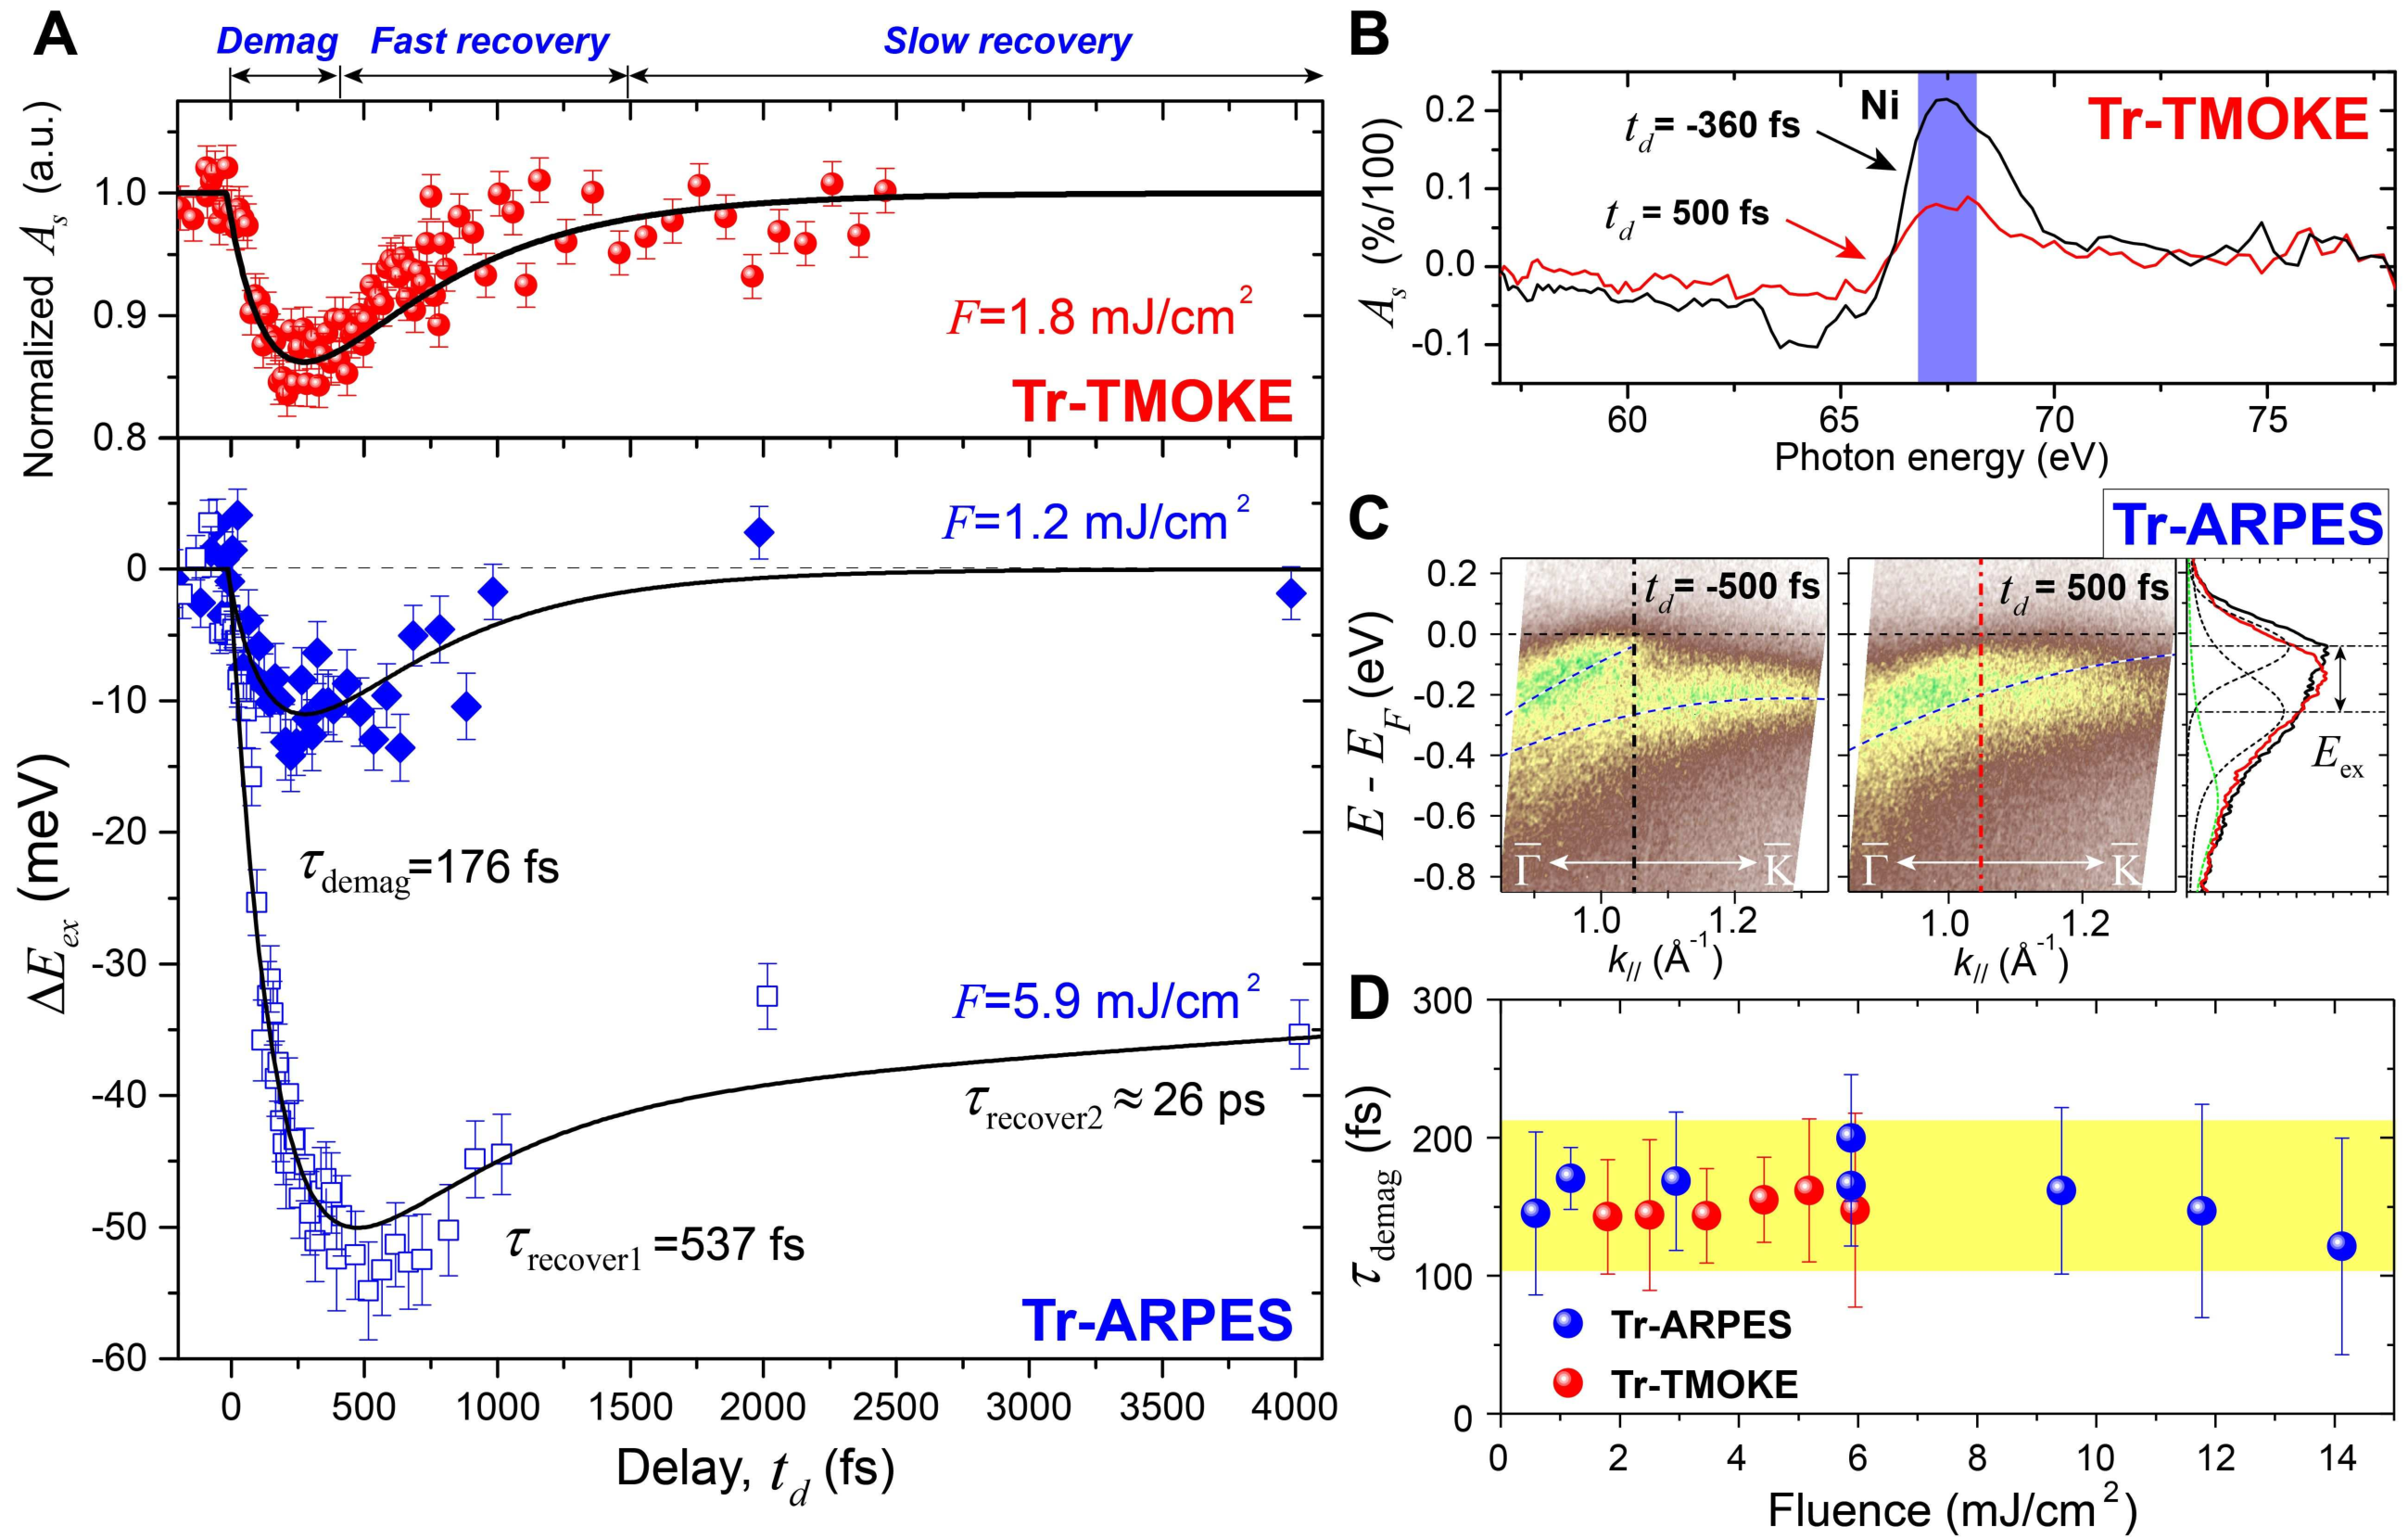
\includegraphics[width=150mm]{aap9744_Figure_fig2_seq2_v1.pdf}
	\end{center}
	\caption{Magnetization dynamics in Ni. (A) Change of the TMOKE asymmetry and exchange splitting reduction $\Delta E_{ex}$ as a function of time delay for different laser fluences. The solid lines represent fitting results, from which we extract the three characteristic times for demagnetization ($\tau_{demag}$), fast recovery ($\tau_{recover1}$), and slow recovery ($tau_{recover2}$) (see Materials and Methods). The fit to TMOKE (upper panel) and ARPES (lower panel and lower fluence) yields the same fluence-independent time constants. a.u., arbitrary units. (B) Typical TMOKE asymmetry before (td = −360 fs) and after (td = 500 fs) excitation with a pump fluence F ≈ 6 mJ/c$m^2$.(C) Photoelectron spectra of Ni(111) along the $\Gamma$ - K direction before ($t_{d}$ = −500 fs) and after ($t_{d}$ = 500 fs) laser excitation, showing the collapse in the exchange splitting $E_{ex}$ after excitation (blue dashed lines). The dashed-dotted lines represent the momentum at which photoemission intensities are extracted. The photoemission intensities are plotted in the right panel with $E_{ex}$ extracted from a Voigt function fit to the data (dashed lines; see the Supplementary Materials). (D) Constant, fluence-independent demagnetization time observed for different laser fluences for both ARPES and TMOKE.}
	\label{fig: Nifig2}
\end{figure}

The dynamics of the exchange-splitting change ($\Delta E_{ex}$)and TMOKE asymmetry ($A_{s}$) can be generally fit by an exponential decay and bi- exponential recovery function (see Materials and Methods). We find that the dynamics of $\Delta E_{ex}$ can be described by a set of time constants, with a dramatic change in recovery times above a critical laser fluence. For all pump laser fluences (below or above the critical fluence), the collapse of the exchange splitting exhibits a constant and fluence- independent time scale of 176 $\pm$ 27 fs. For fluences below a critical laser fluence of $F_{c}$ ≈ 2.8mJ/c$m^2$, the magnetic response exhibits a fast recovery ($\tau_{recover1}$ = 537 $\pm$ 173 fs). For fluences above $F_c$, the magnetic response exhibits the same fast recovery as well as a slower recovery ($\tau_{recover2}$ = 76 $\pm$ 15 ps; see the Supplementary Materials). These characteristic time constants are obtained using a global fitting scheme (see the Supplementary Materials). We note that the minima of dynamics shown in Fig. \ref{fig: Nifig2}A depend on the ratio of demagnetization and fast recovery amplitudes. Although they appear at different time delays for different fluences, the extracted time constants (and characteristic time scales of the processes) are the same. 

To correlate the dynamics of the exchange-splitting collapse $\Delta E_{ex}$ (probed by ARPES) with the laser-induced demagnetization of the sample, we analyze TMOKE measurements taken at similar pump fluences. We find that the time scale of demagnetization measured using TMOKE is the same as the exchange-splitting collapse measured using ARPES and that both are independent of the pump laser fluence (Fig. \ref{fig: Nifig2}D). This is consistent with the conclusion that the collapse of $E_{ex}$ obtained in Tr-ARPES directly represents the quenching of the magnetization in the material, although the dynamics are obtained at a specific momentum. 

In time-resolved ARPES, the dynamic electron temperature can be directly extracted by analyzing the photoemission intensity distribution above $E_{F}$. In Fig. 	\ref{fig: Nifig3}A, we plot the photoemission intensity from above $E_{F}$ at different time delays, for a fluence of 6 mJ/cm$^2$. Before the pump pulse arrives ($t_{d}$ = −500 fs), the photoemission intensity corresponds to a Fermi-Dirac distribution across $E_{F}$ at room temperature. The electron temperature reaches its maximum value at 24 fs after the peak of the pump pulse and then rapidly decreases due to cooling to the lattice. By 2 ps after excitation, the electron temperature is close to room temperature, as evidenced by the fact that the slope of photoemission intensity as a function of energy is very close to that obtained in the ground state ($t_d$ = −500 fs) (Fig. \ref{fig: Nifig3}A). The electron temperature can be reliably extracted by fitting the photoemission intensity with the Fermi-Dirac function convolved with the experimental energy resolution (see the Supplementary Materials). The time evolution of the electron temperature after laser excitation is plotted in Fig. \ref{fig: Nifig3} (B and C). These results are further corroborated by the dynamics of electron population at 0.2 eV (Fig. \ref{fig: Nifig3}B) and the transient EUV reflectivity measurements performed at similar laser fluences (Fig. \ref{fig: Nifig3}C). These measurements probe the charge dynamics around $E_{F}$ averaged over the entire Brillouin zone, by exciting the 3p core level electrons of Ni to electronic states around $E_{F}$ (see inset of Fig. \ref{fig: Nifig3}C). The agreement between the transient electron temperatures extracted from both ARPES and EUV reflectivity measurements suggests that the measured electron dynamics across $E_{F}$ are uniform throughout k-space. The short electron thermalization time in Ni is not surprising if we consider that the lifetime of photoexcited electrons at 1.6 eV above $E_{F}$ is extremely short (1 fs) \cite{Knorren2000}, indicating very strong electron-electron interactions (see Appendix A) \cite{Chen2017}. 
\begin{figure}[htbp]
	\begin{center}
		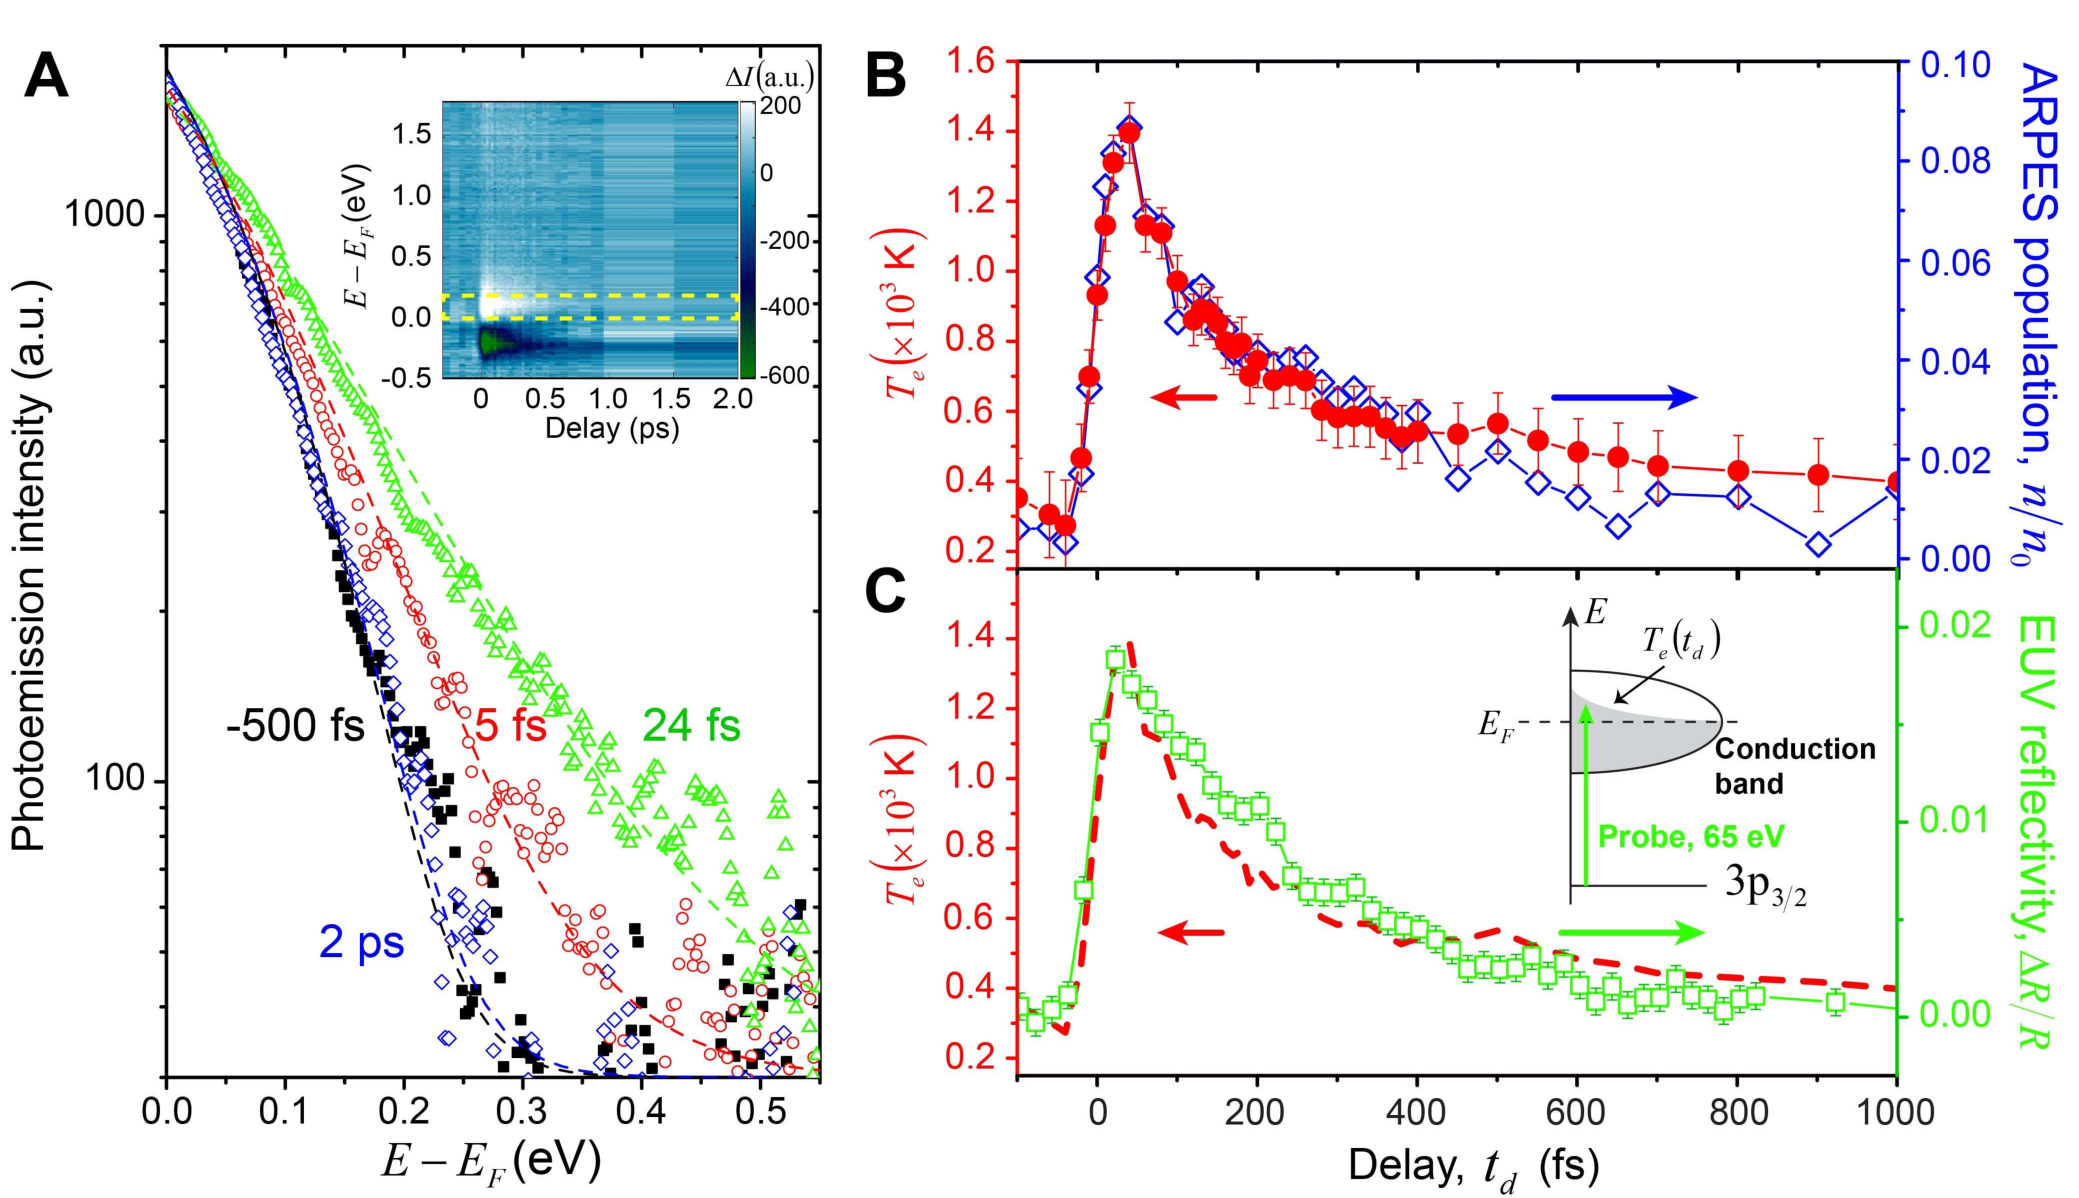
\includegraphics[width=150mm]{aap9744_Figure_fig3_seq3_v1.pdf}
	\end{center}
	\caption{Ultrafast charge dynamics in Ni. (A) Log plots of the photoemission intensity above EF for F ≈ 6 mJ/c$m^2$ and at different td, integrated from $k_{\/\/} \approx 0.85 \AA^{-1}$ to $k_{\/\/} \approx 1.3 \AA^{-1}$ in the momentum space. The dashed lines represent the fitting of the photoemission intensities with the Fermi-Dirac distribution convolved with experimental energy resolution (see the Supplementary Materials). Inset: Integrated photoemission intensity as a function of pump-probe time delay. The yellow dashed box illustrates the integration region of electron population in (B). (B) Dynamics of the electron temperature and the relative electron population (n$\/n_{0}$) within 0.2 eV above $E_{F}$ as a function of $t_d$. The electron population is normalized to the band electron population ($n_{0}$) 0.2 eV below $E_{F}$ (see the Supplementary Materials). (C) Comparison of the electron temperature [red dashed line, same as (B)] and the change of EUV transient reflectivity at a similar pump fluence. Inset: EUV transient reflectivity measurement. The resonant EUV light (65 eV) directly probes the charge dynamics around EF induced by the laser pump pulse. This measurement is averaged over k-space}
	\label{fig: Nifig3}
\end{figure}

In Fig. \ref{fig: Nifig4}A, we plot the maximum electron temperature extracted around 20 fs, which is the characteristic time scale for the rise of the electron temperature after excitation, as a function of the laser pump fluence. Here, we observe the first critical behavior: The increase of the electron temperature is strongly suppressed around the critical fluence $F_{c} \approx$ 2.8 $mJ/cm^2$, indicating that a significant amount of energy is transferred into the spin system within 20 fs, preventing a further increase in electron temperature. The critical behavior of the peak electron temperature (Fig. \ref{fig: Nifig4}A) can be explained by the divergence of the heat capacity of the strongly coupled electron and spin systems in Ni.

\begin{figure}[htbp]
	\begin{center}
		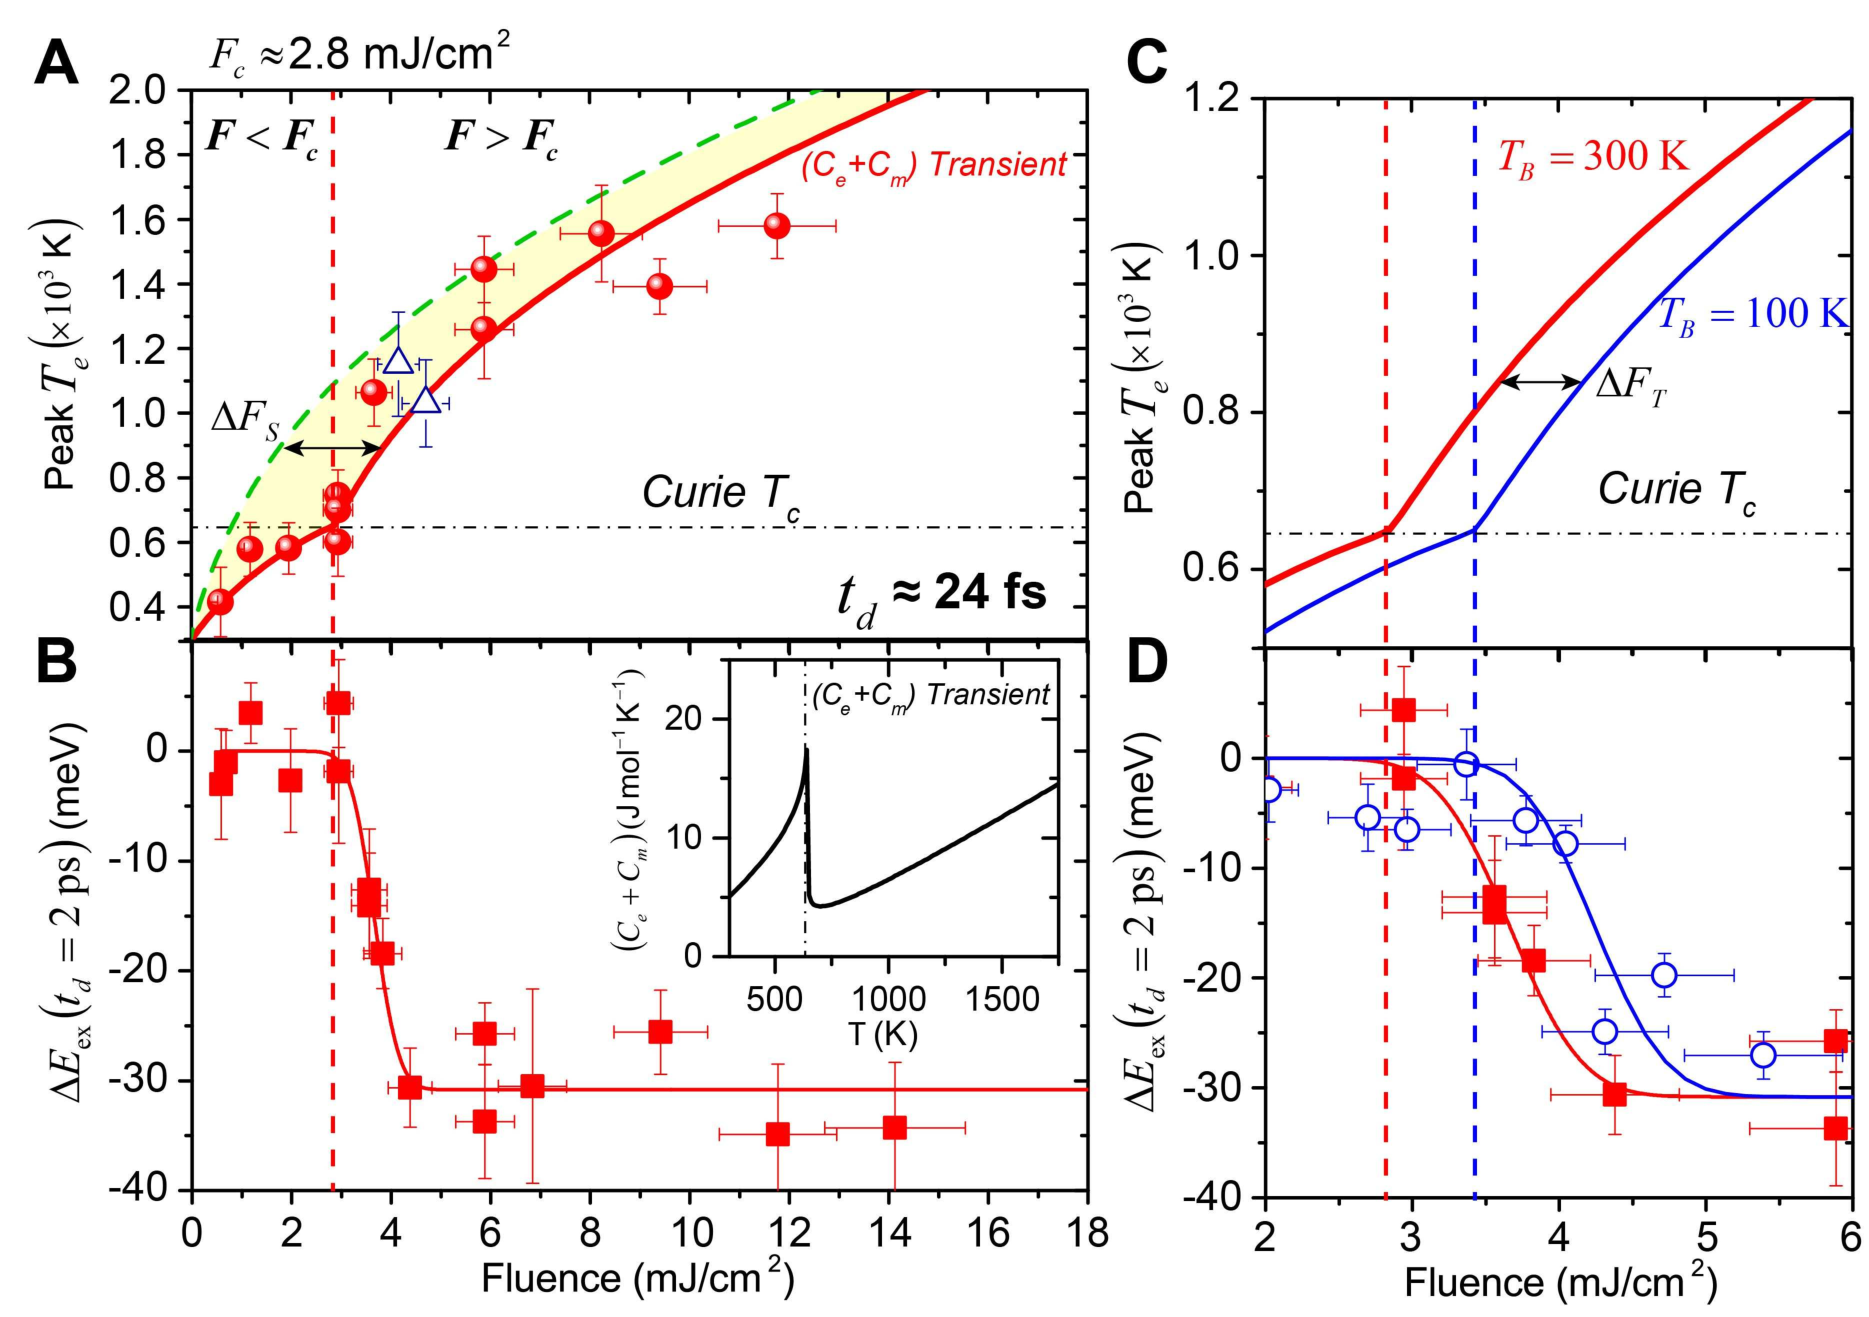
\includegraphics[width=150mm]{aap9744_Figure_fig4_seq4_v1.pdf}
	\end{center}
	\caption{Observation of multiple critical behaviors during ultrafast demagnetization in Ni. (A) Peak electron temperature extracted 24 fs after excitation as a function of pump fluence. The open symbols represent the electron temperature extracted at different k// using Tr-ARPES. The solid red line is the fit using Eq. 1 consider- ing the transient electron and magnetic heat capacity [inset of (B)], whereas the green dashed line considers only the contribution from transient electron heat capacity (see the Supplementary Materials). The yellow-colored region ($\Delta F_{S}$) is the energy transferred to the spin system within 20 fs. (B) Change in the exchange splitting at 2 ps as a function of pump fluence. The red line represents a fit with an error function. The same critical fluence of $F_{c}$ $\approx$ 2.8 mJ/c$m^2$ is observed for the exchange splitting collapse and the peak electron temperature in (A). The transient electron heat capacity is plotted in the inset. (C) Peak electron temperature calculated using Eq. 1 and ($C_{e} + C_{m}$) Transient [inset of (B)] for the sample temperatures of 300 and 100 K. The red solid line is the same as in (A). (D) Change of exchange splitting at 2 ps as a function of laser fluence at different sample temperatures. The solid lines represent the error function fit of the experimental results. The dashed lines align the critical fluences observed in (C) and (D) for different sample temperatures.}
	\label{fig: Nifig4}
\end{figure}

To a first-order approximation, the maximum temperature that the electrons can reach ($T_{max}$) at the sample surface with a given pump fluence (F) can be calculated as:
\begin{equation}
\frac{F(1-R)}{\delta}=\int_{T_{e}^{max}}^{T_{B}}[C_{e}(T)+C_{m}(T)]dT
\label{eqn: 1}
\end{equation}
where R is the reflectivity, d is the penetration depth, $T_{B}$ is the ground state sample temperature, and $C_{e}$ and $C_{m}$ are the heat capacities of the electron and spin systems of Ni, respectively. It is well known that the magnetic heat capacity $C_{m}$ diverges when the temperature approaches the Curie temperature to fulfill the energy required for the ferromagnetic-to-paramagnetic phase transitions under thermal equilibrium conditions \cite{Stohr2006,Meschter1981}(1, 25). Here, we model $C_{e}(T)+C_{m}(T)$ using a power-law function and fit the measured peak electron temperature as a function of pump fluence to Eq.  (see Materials and Methods and the Supplementary Materials). The fitting results are shown as the solid line in Fig. \ref{fig: Nifig4}A, which essentially captures the critical behavior of the peak electron temperature observed in our experiments. The parameters for the optimum fitting are listed in Table 1, whereas the corresponding “transient” heat capacity is plotted in the inset of Fig. \ref{fig: Nifig4}B. We find that the divergence in the heat capacity around the critical temperature ($T_{c}$) can quantitatively explain the critical behavior observed in the electron temperature. $T_{c}$ obtained for the ultrafast transient phase transition is very close to the Curie temperature (see Table 1), which further corroborates that the critical phenomena we observed are related to the intrinsic magnetic properties of Ni. The peak electron temperatures with the contribution of electron heat capacity alone are plotted as the dashed line in Fig. \ref{fig: Nifig4}A (see Materials and Methods and the Supplementary Materials). We estimate that there is an energy of $\Delta E_{s}=\frac{\Delta F_{s}(1-R)}{\delta}\approx$ 105 meV per unit cell transferred to the spin bath within 20 fs. This energy is enough to go through the magnetic phase transition because it is even higher than the energy required under thermal equilibrium conditions (68 meV per unit cell) \cite{Meschter1981}.

As noted above, the slow recovery of the magnetization is only observed when the pump fluence is higher than the same critical fluence $F_{c} \approx$ 2.8mJ/c$m^2$, which represents the second critical behavior. This can be illustrated if we plot the exchange-splitting collapse $\Delta E_{ex}$ at $t_{d}$ = 2 ps as a function of pump laser fluence, as shown in Fig. \ref{fig: Nifig4}B. We note that the observed critical fluence here is consistent with that shown in Fig. \ref{fig: Nifig4}A for the electron temperature, corroborating that the observed critical behavior of the transient electron temperature is related to the laser- induced magnetic phase transition in the spin-electron system. Considering that the electron and lattice temperatures are both less than the Curie temperature of Ni at $t_{d}$ = 2 ps (see below), our results indicate that a transient paramagnetic-like state exists when the pump fluence is above $F_{c}$, which recovers through a path distinctly different from the fast recovery for lower pump laser fluences. We note that the different time scales observed in many magnetic spectroscopy experiments to date \cite{Koopmans2010,Roth2012} can be explained by depth averaging, where parts of the material near the surface undergo a transient magnetic phase transition with slow recovery dynamics, whereas layers deeper within the material exhibit faster recovery dynamics. This was confirmed by comparing an extensive set of fluence-dependent time-resolved ARPES and TMOKE data that show that the same critical behavior can explain the entire data set \cite{You2018}.

To further investigate the driving mechanisms for the observed critical phenomena during ultrafast laser-induced demagnetization, we repeated the same measurements for a sample temperature of 100 K using Tr-ARPES. Figure \ref{fig: Nifig4}D plots the change of exchange splitting at a time delay of 2 ps as a function of pump fluence for sample temperatures of 300 and 100 K. The peak electron temperatures reached for those same sample temperatures are calculated using Eq. 1 and are shown in Fig. \ref{fig: Nifig4}C. For a sample temperature of 100 K, the required critical fluence increases by $\Delta F_{T}$ =0.58mJ/c$m^2$ compared to room temperature (Fig. \ref{fig: Nifig4}D). As shown in Fig. \ref{fig: Nifig4}C, this offset can be precisely captured by Eq. \ref{eqn: 1} using the same transient heat capacity (inset of Fig. \ref{fig: Nifig4}B), thus further validating the extracted value of this transient heat capacity. This result strongly suggests the following criterion for critical behavior in ultrafast demagnetization of Ni: whether or not the transient electron temperature exceeds the Curie temperature. Hence, in our work, the critical fluence corresponds to the fluence required to drive the transient electron temperature above the Curie temperature. We believe that the fact that the critical temperature observed in ultrafast demagnetization is very close to the Curie temperature under thermal equilibrium cannot be a simple coincidence but underscores the importance of the connection between the nonequilibrium physics and its equilibrium counterpart. Similar ideas were recently explored by studies on the ultrafast spin-density-wave transition in Cr \cite{Nicholson2016}. However, in that case, the spin-density-wave phase transition occurs immediately when the transient electron temperature reaches the critical point. In contrast, in our work, critical spin excitations occur within 20 fs, and the ferromagnetic-to-paramagnetic phase transition then happens on a longer time scale that is characteristic of the material. We believe that these mechanisms are broadly applicable to many different materials that undergo phase transitions at a critical temperature, for example, superconductors and charge-density-wave materials.

\section{Discussion}

Our results also shed light on the microscopic time evolution of electron spins during ultrafast demagnetization in Ni. The presence of critical behaviors in the electron temperature and heat capacity shows that, within 20 fs after excitation, the spin system in Ni has already absorbed sufficient energy to go through the ferromagnetic-to-paramagnetic phase transition, without yet exhibiting significant demagnetization. This time scale is much shorter than the time scale of demagnetization (TMOKE) and collapse of the exchange splitting (ARPES) (176 fs). The very large difference between these two time scales indicates the importance of a highly nonequilibrium transient state before the sample reaches maximum demagnetization. The initial transferred energy must be stored in the spin system in the form of high-energy spin excitations, leaving the spin system in a nonequilibrium state. Then, this energy likely decays into low-energy magnons over time, leading to demagnetization of the sample in 176 fs. In this picture, the time scale and critical fluence of the demagnetization is intrinsic to the material itself and is determined by the Curie temperature, heat capacity, and exchange energy. This is strongly supported by the fact that the time constant of demagnetization in Ni (176 fs) is independent of pump laser fluence, as shown by both the Tr-ARPES and Tr-TMOKE measurements (Fig. \ref{fig: Nifig2}D). It has been suggested both experimentally and theoretically that the emission of low-energy magnons on a time scale oftens of femtoseconds could have significant contributions to ultrafast demagnetization in ferromagnetic materials \cite{Carpene2015,Zhang2012,Eschenlohr2013,Schmidt2010,Turgut2016}. Finally, we note that our results cannot be explained by the models based on spin-flip scattering, because, in those models, the demagnetization of the material occurring in several hundred femtoseconds is driven by the gradual transfer of the energy from hot electrons to electron spins via spin-orbit and electron-phonon interactions \cite{Koopmans2009,Krauß2009,Mueller2013,Roth2012}. Moreover, these mechanisms should give rise to a fluence-dependent demagnetization and recovery times.

Now, an important question remains— what is the mechanism that could lead to high-energy spin excitations during the first 20 fs? On this time scale, we believe that superdiffusive spin currents could be an important candidate, considering the significant difference between the lifetimes of the majority and minority electrons at 0.2 eV above EF (10, 11), as well as the extremely short time scale of spin transport (1fs over 1-nm distance). However, it has also been shown both experimentally (31, 32) and theoretically \cite{Tows2015,Krieger2015,Zhang2000} that the spin mixing via spin-orbit coupling can happen in a very short time, which might also contribute.

Furthermore, another interesting finding is that, as evidenced by the critical behavior of $\Delta E_{ex}$ in Fig. \ref{fig: Nifig4}B, because the spin system recovers to the ground-state magnetization, two different recovery regimes exist, depending on the pump fluence. We note that this is the first time that such a critical behavior in the ultrafast decay and recovery time scales has been observed in ferromagnetic metals such as Ni. As noted above, the demagnetization and exchange-splitting collapse times are fluence-independent at 176 fs. However, when the pump fluence is lower than $F_{c}$, we find that the magnetization of the sample undergoes a fast recovery to the ferromagnetic phase with a time constant of 500 fs (Fig. \ref{fig: Nifig2}A). This fast recovery might be explained by damping of magnons (the precession of the magnetic moment M)under the exchange field ($H_{ex}$). The typical damping time is given by $\tau_{damp} = \frac{h}{g\mu_{B}\mu{0}\mid H_{ex}\mid\alpha}$ using the Landau-Lifshiz-Gilbert equation (34, 35), where $\mu_{B}$ is the Bohr magneton, g $\approx$ 2 is the Landé factor, and $\alpha$ is the damping factor. Considering that $\alpha$ = 0.065 (36, 37)and $\mid H_{ex}\mid$ = 939 T for Ni (38), we find $t_{damp}$ $\approx$ 580 fs, which is in quantitative agreement with $\tau_{recover1}$ observed in our experiments. On the other hand, when the pump fluence is above $F_c$, the sample evolves into a transient magnetic state with low magnetization and $H_{ex}$ is melted (see Fig. \ref{fig: Nifig1}A). As a result, the magnetization must recover by coupling to phonons and the lattice, which occurs over much longer times.

In conclusion, by investigating ultrafast laser-induced demagnetization in Ni using fluence- and temperature-dependent ARPES, TMOKE, and EUV transient reflectivity measurements, we unambiguously show that critical phenomena govern the ultrafast demagnetization response. We find that although demagnetization and the collapse of the exchange splitting occur on the same fluence-independent time scale of 176 fs, sufficient energy for the transient magnetic phase transition has been transferred to the spin system already within 20 fs. Our results suggest the existence of a high-energy nonequilibrium transient magnetic state and that the transient electron temperature alone is responsible for crossing the spin electronic phase transition.

\section{Materials and Methods}
\subsection{Experimental setups}
In the ARPES experiment, photoelectrons from the Ni(111) surface are mapped using 16 eV HHG probe pulses at near-normal incidence (5$\deg$) and collected by a momentum-resolved hemispherical analyzer. The output of a Ti:Sapphire laser amplifier system (KM Labs Dragon) is frequency doubled to 390 nm and used to generate high harmonics with 160 meV energy resolution and well-separated (by 6 eV) harmonic orders that allow us to use the fifth harmonic (16 eV) directly (39). For the TMOKE and EUV transient reflectivity experiments, the harmonics are driven directly with the 780-nm laser. Light near HHG orders 43 and 45, at photon energies of 65 and 68 eV, is used to probe the 3p absorption edge of Ni. For this purpose, the HHG probe beam is reflected from the sample at an angle of48° from normal, spectrally dispersed by a grating, and recorded with a charge-coupled device (CCD) camera (9, 11, 30). The sample is fully magnetized in-plane by an electromagnet placed in the transverse geometry (see the Supplementary Materials for more details).

\subsection{Data analysis}
In TMOKE, the sample magnetization is characterized by the change in reflected EUV intensity at the 3p absorption edge for opposite orientations of the initial in-plane magnetization vector. The TMOKE asymmetry ($A_s$) is then calculated from
\begin{equation}
A_{s}=\frac{I_{+}-I_{-}}{I_{+}+I_{-}}
\label{eqn:2}
\end{equation}
where $I_+$ and $I_−$ are the reflected EUV intensities for two magnetization directions \cite{La-O-Vorakiat2012,Mathias2012,La-O-Vorakiat2009}. Details of data analysis of ARPES experiments are presented in detail in the Supplementary Materials. The dynamics of TMOKE asymmetry ($A_s$) and change of the exchange splitting ($\Delta E_{ex}$) can both be fit to
\begin{equation*}
Y(t_{d}) = 
\begin{cases}
Y_0 \\
Y_0 + a e^{-t_d\/\tau_{demag}}-b e^{-t_d\/\tau_{recover1}}-(a-b)e^{-t_d\/\tau_{recover2}}
\end{cases}
\label{eqn:3}
\end{equation*} 
where Y represents either $\Delta E_{ex}$ or $A_s$, $Y_0$ is the ground-state signal, and a and b are the amplitudes of the collapse and the first fast recovery of the signal, respectively. $\tau_{demag}$, $\tau_{recover1}$,and $\tau_{recover2}$ are the time constants of the collapse, fast recovery, and slow recovery of the signal, respectively.

\subsection{Model of electronic and magnetic heat capacity}
The electronic and magnetic heat capacity $C_e(T)+ C_m(T)$ can be modeled with the following power-law function as it passes through the critical temperature ($T_c$) \cite{Kornblit1975}
\begin{equation}
C_{e}(t)+C_m(t) = \frac{A}{\beta}|t^{-\beta}| + B + \gamma t
\label{eqn:4}
\end{equation}
where $t=\frac{T-T_{c}}{T_c}$ is the reduced temperature for T $> T_c$. We used the same function with primed parameters (A', B') for T $< T_c$. The parameters b, $\gamma$, and $T_c$ are kept identical on both sides of the phase transition. The electronic and magnetic heat capacities under thermal equilibrium conditions (25) can be fit to Eq. \ref{eqn:4}, allowing us to extract parameters A, A′, and b, which determine the critical behavior of the heat capacities around $T_c$. The contribution of the electron heat capacity alone can be estimated under the free-electron gas approximation $C_e$ = $\gamma$’T (see the Supplementary Materials) and gives rise to the modeled peak electron temperature using Eq. \ref{eqn: 1}, as shown by the dashed line in Fig. \ref{fig: Nifig4}A. We also noted that in Eq. \ref{eqn: 1}, we neglected electron-phonon coupling and heat diffusion; however, these effects have negligible influence on our results in the first 20 fs, as shown in Appendix A.

\subsection{Statistical analysis}
In both Tr-ARPES and Tr-TMOKE experiments, the data were collected with multiple pump-probe delay cycles to achieve a sufficient signal-to-noise ratio. The exchange splitting dynamics were analyzed by fitting the extracted photoemission spectra with multiple Voigt functions and defined as the energy difference between peaks of electrons with majority and minority spins (see the Supplementary Materials for more details). The error bars in Figs. \ref{fig: Nifig2}A and \ref{fig: Nifig4} (B and D) were due to uncertainties in the fitting procedure. The transient electron temperature was obtained by fitting the photoemission intensity above $E_{F}$ with Fermi-Dirac distribution, and the error bars in Figs. \ref{fig: Nifig3}B and \ref{fig: Nifig4}A were due to uncertainties in the fitting procedure, as well as the energy resolution (see the Supplementary Materials). The errors on the pump fluence were due to fluctuations of pump power and laser spot size. The error bars of Tr-TMOKE data in Fig. \ref{fig: Nifig2} (A and D) were defined by the standard deviation of experimental data before pump excitation.

\subsection{Details of experimental setups}
The detailed experimental setup of Tr-ARPES is shown in fig. S1A. We use a multi-pass Ti:Sapphire laser system to generate 28 fs pulses at a wavelength of 780 nm (1.6 eV) with pulse energy of 2.0 mJ and a repetition rate of 4 kHz. Most of the laser energy (95\%) is used for high-harmonic generation (HHG), while a small portion (5\%) is used to excite the sample as the pump. To generate HHG, we send 95\% of the laser power into a 200 $\mu$m thick $\beta$-phase barium borate (BBO) crystal, which produces pulses at a wavelength of $\approx$390 nm with pulse energy $\approx$ 0.3 mJ. The residual 780 nm light is removed from the beam path using two dichroic mirrors after the BBO. The 390 nm light is then focused using a lens with 50 cm focal distance into a 1-cm-long capillary waveguide. The waveguide has an inner diameter of 150 $\mu$m and is filled with Xe at a pressure of $\approx$20 Torr or Kr at a pressure of $\approx$60 Torr. The HHG beam is focused onto the nickel sample in the UHV chamber using a toroidal BK7 mirror to a spot size of $\approx$100 μm in full width of half maximum (FWHM). Any residual driving laser light is blocked by a 200 nm thick polycrystalline Al filter. The excited photoelectrons are collected by a hemispherical electron analyzer. The energy resolution is calibrated using the photoemission spectrum from a polycrystalline Cu at the room temperature and yields $\approx$160 meV. For ARPES, the atomically clean Ni(111) surface is obtained in-situ using repeated cycles of Argon ion sputtering (0.5 keV) at room temperature, followed by annealing to 900 K for 15 minutes.

The linearly polarized 780 nm pump beam is recombined collinearly with the HHG beam using an annular silver mirror and focused onto the sample surface. The pump fluence is varied by the combination of a half waveplate and a polarizer, as shown in Fig. \ref{fig: NiSIfig1}A. The pulse durations of the pump-probe experiment is directly measured in-situ using the laser-assisted photoemission (LAPE) method. In the LAPE measurement, p-polarized pump light is focused onto the sample surface. When the pump pulse temporally overlaps with the HHG-probe pulse, a side band can be clearly observed at an energy 1.6 eV away from the main photoemission peak, which allows us to extract the cross-correlation of the pump and probe pulses. The side band intensity as a function of td obtained from LAPE measurement is shown in fig. S1B. We note that in order to avoid the influence of LAPE signals on our measurements of ultrafast charge and exchanging splitting dynamics, we switch to s-polarized IR pump in the other two measurements.

In both experiments, the spot sizes of pump are measured using the knife-edge method in-situ at the sample location. The pump fluence in this work is defined as $F=\frac{4Q}{\pi D_x D_y}$ , where Q the is the pump-pulse energy and $D_{x/y}$ is the FWHM of the pump spot along two orthogonal axes. In order to compare the fluence-dependent results between two experiments, the difference in the reflectivity at different incident angles has to be taken into consideration. According to the optical constants of Ni (43), the reflectivity R at normal incidence is $\approx$0.74, which changes to $\approx$0.64 for the p-polarized pump at an incident angle of 48 degrees measured with respect to the normal. This value is also confirmed by reflectivity measurement on site. The fluence reported in the main text for Tr-TMOKE results are scaled considering this difference to preserve the same absorbed fluence as that in Tr-ARPES measurements. In both experiments, the time solution is estimated to be $\approx$10 fs, considering the fastest changes that can be observed from the data.

\begin{figure}[htbp]
	\begin{center}
		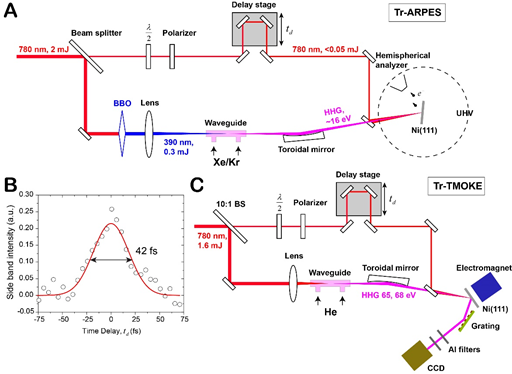
\includegraphics[width=150mm]{figs/NiFigS1}
	\end{center}
	\caption{Experimental Setup. (A) Experimental setup of Tr-ARPES experiment. (B) Side band intensity as a function of pump-probe time delay in LAPE measurement for Tr-ARPES. The solid line is the fitting result with the Gaussian function with a FWHM of $\approx$42 fs. (C) Experimental setup of Tr-TMOKE experiment.}
	\label{fig: NiSIfig1}
\end{figure}

\subsection{Method for extracting TMOKE asymmetry dynamics from HHG spectra}
In the Tr-TMOKE experiment, to extract the asymmetry dynamics at the nickel edge, we use a spectrometer as shown in Fig. \ref{fig: NiSIfig1}C. We take an average of the signal over an energy range of the spectrometer approximately equal to 1.2 eV for each harmonic, although we note that this width is also convolved with the spot size of the HHG beam after reflection off the grating. We select the harmonics corresponding to the 43rd and 45th harmonic of the fundamental laser (corresponding to energies of 65 and 68 eV) in the data analysis procedure. Finally, we normalize the data before the pump pulse arrives by taking the average value of the static asymmetry. We use the standard deviation in values for static asymmetry measured before the sample is pumped to determine the error bars for the TMOKE measurement.

\subsection{Momentum dependence of TMOKE Measurements}
In order to investigate the momentum dependence of the Tr-TMOKE measurements, we took several different time-resolved asymmetry measurements with different crystal lattice orientations relative to the applied field B, with an incident pump fluence of 2.8 mJ/c$m^2$. These measurements are shown in Fig. \ref{fig: NiSIfig7}. These results clearly show the momentum-averaged nature of the Tr-TMOKE measurement.

\begin{figure}[htbp]
	\begin{center}
		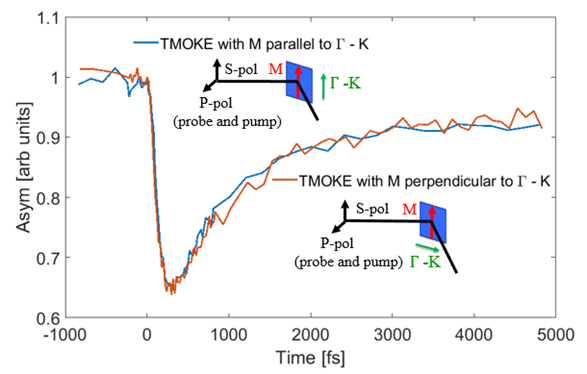
\includegraphics[width=150mm]{figs/NiFigS7}
	\end{center}
	\caption{Momentum dependence of TMOKE measurements. The TMOKE asymmetry dynamics for different crystal orientations. Inset:  Illustrations of the relative orientations of the crystal cut relative to the directions of the magnetic field and light polarizations in the experimental geometry.}
	\label{fig: NiSIfig7}
\end{figure}

\subsection{Transient electron and magnetic heat capacity}
The electron and magnetic heat capacity is modeled using Eq. \ref{eqn:4} with six parameters (A, A', B, B', $\beta$, $\gamma$ and $T_c$). In order to reduce the number of free fitting parameters, we first determine the values of A, A' and $\beta$ by fitting the electron and magnetic heat capacity under thermal equilibrium (25) to Eq. \ref{eqn:4}. The fitting results are plotted in Fig. \ref{fig: NiSIfig8}A. By doing so, we assume the order parameters for the critical behavior of heat capacities are preserved in laser-induced phase transition. At the same time, the fact that the total heat capacity at T=0 is zero places an additional confinement on the parameters: $\frac{A'}{\beta}$ + B'$\gamma$=0. As a result, we have in total three free fitting parameters when we fit the experimentally measured $T_e$ (Fig. \ref{fig: Nifig4}) to Eqs. \ref{eqn:3} and \ref{eqn:4}. 
The critical behavior of the nickel heat capacity represents the energy transfer into the spin bath when the system crosses the ferromagnetic-to-paramagnetic phase transition. In transient ($C_e+C_m$), the contributions of the electron heat capacity can be estimated under the free-electron-gas approximation: $C_e=\gamma'T$ , as shown in Fig. \ref{fig: NiSIfig8}B. We note that when T $<$ $T_c$, $\gamma$' is close to the value for thermal equilibrium (25). However, we find $\gamma$' is about 3 times larger than its thermal equilibrium counterpart when T $>$ $T_c$, the reason of which requires further investigations. Using the transient $C_e$ and Eq.\ref{eqn:3} in the main text, we can estimate the peak electron temperature without spin contributions, which is shown as the pink dashed line in Fig. \ref{fig: Nifig4}A. The offset in fluence of this curve to the experimentally measured peak electron temperature represents the amount of pump energy ($\Delta F_S$) transferred to the electron spin bath in $\approx$20 fs.  

\begin{figure}[htbp]
	\begin{center}
		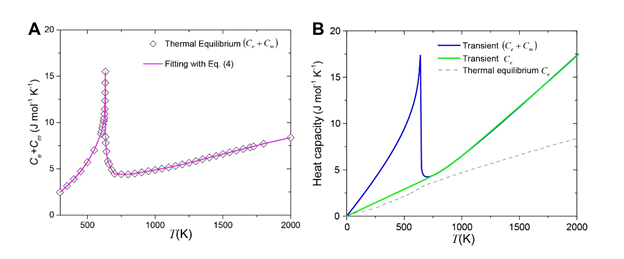
\includegraphics[width=150mm]{figs/NiFigS8}
	\end{center}
	\caption{Electron and spin heat capacity. (A) The electron and magnetic heat capacity under thermal equilibrium (25). The solid line is the fitting result to Eq. (4) in the main text. (B) The transient electron and magnetic heat capacity extracted from our experimental results. The green line represents the contribution of the electron bath to the total heat capacity. The dashed line is the electron heat capacity under thermal equilibrium for comparison (25). }
	\label{fig: NiSIfig8}
\end{figure}

\subsection{Effects of electron-phonon coupling and heat diffusion on Eq. \ref{eqn: 1}}
In Eq. \ref{eqn: 1}, we ignored the heat diffusion and electron-phonon coupling that could reduce the electron temperature at the surface measured using Tr-ARPES method. These two effects can be explicitly considered using two-temperature model (TTM)(47). The time (t)- and space (z)-dependent evolution of the electron ($T_e$) and lattice temperatures ($T_l$) is described by
\begin{eqnarray*}
C_{em}-\frac{\partial T_e}{\partial t}=-\frac{\partial}{\partial z} Q_e - G(T_e-T_l)+S(z,t)\\
\tau_e\frac{\partial Q_e}{\partial t}+Q_e=\kappa_e \frac{\partial}{\partial z}T_e \\
C_l \frac{\partial T_l}{\partial t} = G(T_e - T_l)
\label{eqn:S3}
\end{eqnarray*}
where $Q_e$ is the heat flux of electrons, G the electron-phonon (e-ph) coupling constant, $\tau_e$ the electron energy relaxation time, $\kappa_e = \kappa_{e0}\frac{T_e}{T_l}$ the electron thermal conductivity and $C_l$ the lattice heat capacity. In Eq. \ref{eqn:S3}, the heat diffusion through lattice is neglected, because the lattice thermal conductivity ($\kappa_l$) is much smaller than $\kappa_e$. The values of $\tau_3$, $\kappa_{e0}$ and $C_l$ of Ni can be determined by previous literature(48) as well as material parameters, and are listed in Table S1. We note that $\tau_e$  varies from $\approx$20 fs to 1 fs as the electron energy rises from 0.2 eV to 1.5 eV above $E_F$ (23). This value is shorter than the pump pulse duration ($\approx$28 fs). As a result, the dynamics of electron and lattice temperature have very weak dependence on the choice of $\tau_e$. For convenience, we use $\tau_e$= 10 fs in all the simulations. In Eq. \ref{eqn:S3}, the pump laser pulse is modeled as
\begin{equation}
S(z,t)=\sqrt{\frac{4 \log{2}}{\pi}}\frac{(1-R)F}{t_p\delta}\times exp \left[-\frac{z}{\delta}-4\log{2} \left( \frac{t}{t_p} \right)^2 \right]
\label{eqn:S4}
\end{equation}
where F is the pump fluence, R the reflectivity, $\delta$ the IR-light penetration depth and $t_p$ the pump pulse FWHM width. The values of $\delta$ and $t_p$ are also listed in Table S1.
The heat capacity $C_{em}$ in Eq. \ref{eqn:S3} is defined as the total heat capacity of the electron and spin systems ($C_e+C_m$). In the simulation, we use the temperature-dependent transient ($C_e+C_m$) as plotted in the inset of Fig. \ref{fig: Nifig4}B. This choice is validated by the fact that the electron and spin systems are found to be strongly coupled in short time after pump excitation, evidenced by the critical behavior of the electron temperature at $\approx$24 fs as shown in Fig. \ref{fig: Nifig4}A. The coupled differential equations in Eqs. \ref{eqn:S3} and \ref{eqn:S4} are numerically solved using MacCormack method. In Fig. \ref{fig: NiSIfig9}A, the simulation results of $T_e$ averaged over 1 nm under the sample surface are plotted in direct comparison with the electron temperature measured using Tr-ARPES in our experiments. We find very good agreement can be achieved for a range of pump fluence when a proper temperature dependent e-ph coupling constant G is implemented. The value we used here is a factor of 3 stronger than values reported in Ref. \cite{Lin2008}.  Very interestingly, we find the TTM simulations results show that there exists a “kink” in the recovery dynamics of the electron temperature, whenever the electron temperature reduces to the critical temperature. This reproduces our experimental data very well, which in the time domain strongly supports that the transient electron and magnetic heat capacity influences the laser-induced dynamics. On the other hand, in order to account for the dynamics of the EUV reflectivity, the electron temperature averaged across the EUV probing depth ($\approx$10 nm) has to be taken into consideration, as shown in Fig. \ref{fig: NiSIfig9}B.

The calculations using TTM also allow us to investigate the contributions from heat diffusion and electron-phonon coupling to the model in Eq. \ref{eqn: 1}. In Fig. \ref{fig: NiSIfig9}C, we plot the $T_e$ obtained from TTM simulation for 1) thermally isolated, same as Eq. \ref{eqn: 1}, by setting $\kappa_e$ = 0 and G = 0, 2) heat diffusion only, by setting G=0 and $\kappa_e$ $\neq$ 0 and 3) heat diffusion and e-ph coupling with G $\neq$ 0 and $\kappa_e$ $\neq$ 0. From the results, we can see that the surface electron temperature could be reduced by less than 100 K within 20 fs through heat diffusion when the sample is pumped by a relatively high fluence (5.8 mJ/c$m^2$). This value is expected to be much smaller at lower pump fluences. In contract, the e-ph coupling has negligible effects on electron temperature in 20 fs, because the characteristic time of e-ph coupling is on a time scale of $\approx$100 fs. At the same time, we can also investigate whether the convolution with the time-resolution of our measurement could affect the electron temperature measurements (dashed line in Fig. \ref{fig: NiSIfig9}C). We find the time resolution of our experiment is sufficient to precisely capture the electron temperature in very short time scales.

\begin{figure}[htbp]
	\begin{center}
		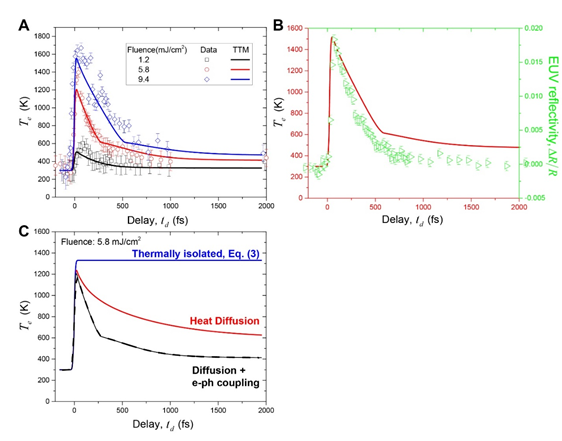
\includegraphics[width=150mm]{figs/NiFigS9}
	\end{center}
	\caption{Two-temperature model. (A) The electron temperature measured using Tr-ARPES in comparison with the simulation results from TTM for the top 1nm thick layer of Ni with different pump fluence. (B) The transient EUV reflectivity results in comparison with the TTM simulation considering the average over a EUV probing depth of $\approx$10 nm. (C) The electron temperature simulated by TTM considering the situations: 1) thermally isolated, same as Eq. \ref{eqn: 1}; 2) only heat diffusion; 3) heat diffusion + e-ph coupling. The dashed line represents the simulation results convolved with the experimental time resolution. }
	\label{fig: NiSIfig9}
\end{figure}